% THIS IS SIGPROC-SP.TEX - VERSION 3.1
% WORKS WITH V3.2SP OF ACM_PROC_ARTICLE-SP.CLS
% APRIL 2009
%
% It is an example file showing how to use the 'acm_proc_article-sp.cls' V3.2SP
% LaTeX2e document class file for Conference Proceedings submissions.
% ----------------------------------------------------------------------------------------------------------------
% This .tex file (and associated .cls V3.2SP) *DOES NOT* produce:
%       1) The Permission Statement
%       2) The Conference (location) Info information
%       3) The Copyright Line with ACM data
%       4) Page numbering
% ---------------------------------------------------------------------------------------------------------------
% It is an example which *does* use the .bib file (from which the .bbl file
% is produced).
% REMEMBER HOWEVER: After having produced the .bbl file,
% and prior to final submission,
% you need to 'insert'  your .bbl file into your source .tex file so as to provide
% ONE 'self-contained' source file.
%
% Questions regarding SIGS should be sent to
% Adrienne Griscti ---> griscti@acm.org
%
% Questions/suggestions regarding the guidelines, .tex and .cls files, etc. to
% Gerald Murray ---> murray@hq.acm.org
%
% For tracking purposes - this is V3.1SP - APRIL 2009

\documentclass{acm_proc_article-sp}

\usepackage{hyperref}

\begin{document}

\title{GLR-based Abstract Parsing}


%
% You need the command \numberofauthors to handle the 'placement
% and alignment' of the authors beneath the title.
%
% For aesthetic reasons, we recommend 'three authors at a time'
% i.e. three 'name/affiliation blocks' be placed beneath the title.
%
% NOTE: You are NOT restricted in how many 'rows' of
% "name/affiliations" may appear. We just ask that you restrict
% the number of 'columns' toio three.
%
% Because of the available 'opening page real-estate'
% we ask you to refrain from putting more than six authors
% (two rows with three columns) beneath the article title.
% More than six makes the first-page appear very cluttered indeed.
%
% Use the \alignauthor commands to handle the names
% and affiliations for an 'aesthetic maximum' of six authors.
% Add names, affiliations, addresses for
% the seventh etc. author(s) as the argument for the
% \additionalauthors command.
% These 'additional authors' will be output/set for you
% without further effort on your part as the last section in
% the body of your article BEFORE References or any Appendices.

\numberofauthors{2} %  in this sample file, there are a *total*
% of EIGHT authors. SIX appear on the 'first-page' (for formatting
% reasons) and the remaining two appear in the \additionalauthors section.
%
\author{
% You can go ahead and credit any number of authors here,
% e.g. one 'row of three' or two rows (consisting of one row of three
% and a second row of one, two or three).
%
% The command \alignauthor (no curly braces needed) should
% precede each author name, affiliation/snail-mail address and
% e-mail address. Additionally, tag each line of
% affiliation/address with \affaddr, and tag the
% e-mail address with \email.
%
% 1st. author
\alignauthor
Semen Grigorev\\
       \affaddr{St. Petersburg State University}\\
       \affaddr{198504, Universitetsky prospekt 28}\\
       \affaddr{Peterhof, St. Petersburg, Russia.}\\
       \email{rsdpisuy@gmail.com}
% 2nd. author
\alignauthor
Iakov Kirilenko\\
       \affaddr{St. Petersburg State University}\\
       \affaddr{198504, Universitetsky prospekt 28}\\
       \affaddr{Peterhof, St. Petersburg, Russia.}\\
       \email{jake@math.spbu.ru}
}
% There's nothing stopping you putting the seventh, eighth, etc.
% author on the opening page (as the 'third row') but we ask,
% for aesthetic reasons that you place these 'additional authors'
% in the \additional authors block, viz.
%\additionalauthors{Additional authors: John Smith (The Th{\o}rv{\"a}ld Group,
%email: {\texttt{jsmith@affiliation.org}}) and Julius P.~Kumquat
%(The Kumquat Consortium, email: {\texttt{jpkumquat@consortium.net}}).}
%\date{30 July 1999}
% Just remember to make sure that the TOTAL number of authors
% is the number that will appear on the first page PLUS the
% number that will appear in the \additionalauthors section.

\maketitle
\begin{abstract}

Abstract parsing is an important step of the processing of dynamically constructed statements or string-embedded languages (such as embedded or dynamic SQL). Existing LALR-based algorithms have performance issues. To increase performance we propose to use a GLR-algorithm as a base for abstract parsing and to reuse graph-structured stack and shared packed parse forest. RNGLR-algorithm modification for abstract parsing is presented. 

\end{abstract}

% A category with the (minimum) three required fields
\category{D.3.4}{Programming Languages}{Processors}[parsing]
\category{D.2.7}{Software Engineering}{Distribution, Maintenance, and Enhancement}[Restructuring, reverse engineering, and reengineering]
%A category including the fourth, optional field follows...
%\category{D.2.8}{Software Engineering}{Metrics}[complexity measures, performance measures]

\terms{Algorithms, Parsing}

\keywords{Dynamic SQL, GLR, RNGLR, abstract parsing, embedded languages, string-embedded languages, two-staged languages, injected languages, abstract translation} % NOT required for Proceedings

%: \href{http://2012.secr.ru/lang/en-en/ \\ talks/dynamic-sql-transformation-automatization}{http://2012.secr.ru/lang/en-en/talks/dynamic-sql- \\ transformation-automatization}}.

\section{Introduction}

Abstract parsing~\cite{Doh:2009:APS:1615441.1615461} is an important step of solutions for dynamically generated statements processing such  as static errors checking, translation, and string-embedded languages support in IDE. Practice experience of abstract analysis implementation as part of dynamic SQL~\cite{SQLISO} translation shows that  exponential resources are required~\cite{GrigorevDSQL} if semantic calculation is necessary. This fact often makes it impossible to process the code of real-world systems. In order to improve analysis performance we have suggested the solution based on dynamic filtration of the parsing results\footnote{Solution was presented at the CEE-SECR 2012.} However, this solution has some critical problems with semantic calculation correctness, besides, performance improvements is not enough for interactive processing in IDE.

Most abstract parsing implementation -- such as PHP String Analyzer~\cite{Minamide:2005:SAD:1060745.1060809} or Alvor\footnote{Alvor project site: \href{http://code.google.com/p/alvor/}{http://code.google.com/p/alvor/}}~\cite{AlvorConf,Annamaa:2010:ITA:1947873.1947886} -- are based on LR or GLR parsing algorithm~\cite{Grune:2010:PTP:1951778} and require additional data structures to store state data which lead to a big memory consumption in case of supporting semantics. It is possible to improve performance and to reduce memory consumption by using GLR-algorithm, extended with support of branching in the input graph, as the base for algorithm of analysis. We can also achieve this aim by means of graph-structured stack (GSS) and the intermediate representation of parsing results reusing.

In this work we present abstract parsing algorithm based on modified RNGLR-algorithm~\cite{Scott:2006:RNG:1146809.1146810} and  the generator of the corresponding parsers. We also describe the main points of the algorithm and the basic aspects of the implementation. Described algorithm is implemented as a part of YaccConstructor\footnote{YaccConstructor project site: \href{http://recursive-ascent.googlecode.com}{http://recursive-ascent.googlecode.com}}~\cite{GrigorevKirilenkoYC} project -- an open source framework for research and development of parser generators, compiler-compilers and other grammarware for .NET. In addition to this, we present some examples which demonstrate dynamically generated statements processing using suggested algorithm.

\section{Related Work}

Most practical tasks require not just parsing, which check whether input is in specified language, but also the ability of various parsing results transformations. There are abstract parsing and abstract lexing for string-embedded languages processing~\cite{Doh:2009:APS:1615441.1615461}. But these algorithms are not applicable for transformation as they skip information about the initial source code positions of the tokens produced from embedded statements, which makes it impossible to modify the original code. Moreover parsing does not include semantic calculation which is required for translation and number of other transformations. However this kind of parsing can be useful for the errors checking or improvements of the code analysis of the whole system.
 
Dynamically constructed queries in the real-world systems have a high complexity so it is very important to improve analysis performance. Implementation of query constructing may contains more than dozens of assignments and conditional branchings~\cite{GrigorevDSQL}. Generally, the algorithm directly based on abstract parsing require an exponential resources. Algorithm for dynamic filtration of syntax analysis results was proposed in work~\cite{GrigorevDSQL}. The approach described in it can significantly reduce forest size for complex queries. But suggested algorithm has a number of problems with semantic calculation correctness. Moreover not all of the performance issues were solved.

\subsection{Abstract Parsing Algorithm}

Abstract parsing is one of the algorithms for syntax analysis of such generalized representation of strings set as data-flow equation or regular expression~\cite{Doh:2009:APS:1615441.1615461}. For practical use we often suppose that the compact representation of the set being processed is a graph. Each edge of this graph contains a token and each vertex corresponds to the concatenation of statement parts. The following example illustrates it. Here you can see the code sample in which some dynamic query is constructed:

\begin{verbatim} 
(1) IF @X = @Y
(2) SET @TABLE = '#tbl1'
(3) ELSE
(4) SET @TABLE = 'tbl2'
(5) SET @S = 'SELECT x FROM ' + @TABLE
(6) EXECUTE (@S)
\end{verbatim}

Variable \verb @S \ contains dynamically generated query and has 2 possible values at the point of query execution. During approximation we can get a graph which presents the set of the possible values of the variable \verb @S \ at the line 6. This graph is presented in figure~\ref{pic1}.


\begin{figure*}
    \centering
    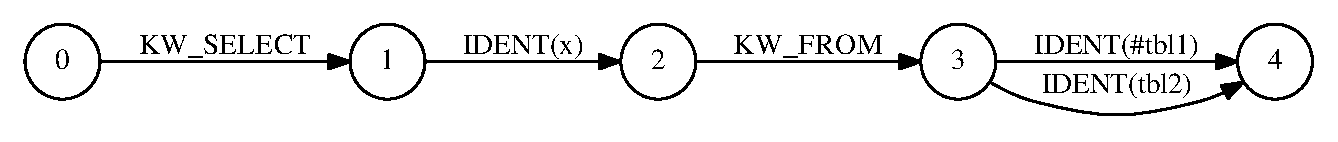
\epsfig{file=graphs/simple_sql.eps, height=1.5cm, width=0.8\textwidth}
    \caption{Graph for dynamic query.}
    \label{pic1}
\end{figure*}


Abstract parsing is based on the idea of reusing of the control structures utilized in the classical parsing with the implementation of special mechanism of their interpretation. Control tables for the analyser (action, goto) may be generated by the language specification by using some standard tool i.e. Yacc. LR automaton~\cite{Grune:2010:PTP:1951778} should be modified so that it is able to compute all possible parser states for each vertex of the graph~\cite{Doh:2009:APS:1615441.1615461}. So, the basic idea of the abstract parsing is a graph processing with fix-point calculation~\cite{AlvorConf}.

Suppose that the grammar of language is the following:

\begin{verbatim} 
s -> Ae
e -> BD
e -> CD
\end{verbatim}
 
Input graph for analyzer, which was generated by the specified grammar, is presented in the figure~\ref{pic2}.

\begin{figure}
    \centering
    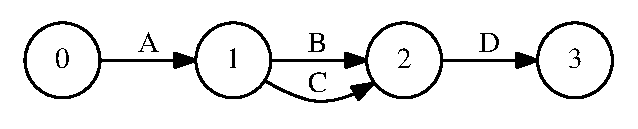
\epsfig{file=graphs/simple_grammar_inpt.eps, height=1cm, width=0.5\textwidth}
    \caption{Input graph for abstract parsing.}
    \label{pic2}
\end{figure}

During syntax analysis the set of the parser states should be calculated for each vertex of the graph. States calculation result is shown in figure~\ref{pic3}.
 
\begin{figure*}
    \centering
    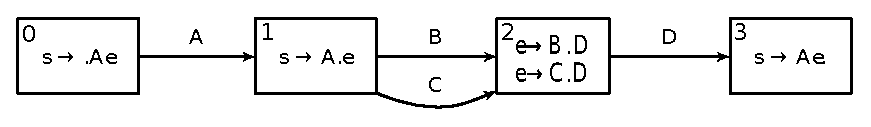
\epsfig{file=graphs/simple_grammar_items.eps, height=1.6cm, width=0.8\textwidth}
    \caption{Parser states for graph in figure~\ref{pic2}.}
    \label{pic3}
\end{figure*}


\subsection{Tools for Static Analysis of Dynamic Statements}

Many tools use dynamically generated queries for communicating with databases. This leads to the fact that safety assurance and quality of work for real-world systems is very difficult. So static processing of dynamically generated strings is an important problem. One of the most popular area is string-embedded SQL processing: static errors detection, SQL injections vulnerabilities detection~\cite{Fu:2007:SAF:1299135.1299784}. Tools for Web-pages (HTML) generation also exist.

The following tools can be used for dynamically generated SQL queries processing:

\begin{itemize}
\item Java String Analyzer (JSA)~\cite{JSAArticle} is a tool for analyzing the flow of strings and string operations in Java programs. For each string expression, it computes a finite-state automaton that provides an upper approximation of the values that may appear at runtime.

\item  Alvor~\cite{Annamaa:2010:ITA:1947873.1947886}  is an Eclipse plug-in, which statically validates SQL sentences embedded in Java code. It can be used either as one-shot full-program analyzer or as incremental as-you-type error guard. SQL strings found in the code can be checked against built-in SQL grammar or against actual test database.

\item  PHP String Analyzer (Phasa)\footnote{PHP String Analyzer project site: \href{http://www.score.is.tsukuba.ac.jp/~minamide/phpsa/}{http://www.score.is.tsukuba.ac.jp/$\sim$minamide/phpsa/}}~\cite{Minamide:2005:SAD:1060745.1060809}  is a static program analyzer that approximates the string output of a PHP program with a context-free grammar. The analyzer can be used to check properties of a PHP program. For example, it can be used to validate dynamically generated Web pages by a PHP program.

\item SAFELI~\cite{Fu:2007:SAF:1299135.1299784} is a static analysis framework for identifying SQL injection attack vulnerabilities at compile time. SAFELI statically inspects MSIL bytecode of an ASP.NET Web application.

\item A Static Analysis Framework for Database Applications~\cite{Dasgupta:2009:SAF:1546683.1547548} is a framework which can analyze database  application binaries that use ADO.NET data access APIs. It can be used for a variety of analysis tasks such as SQL injection detection, workload extraction, identifying performance problems, and verifying data integrity constraints in the application. 
\end{itemize}

Most of tools use LR-based abstract parsing as a core of the algorithm. Alvor uses some ideas from GLR-algorithm for stack organization. However, some additional data structures are required during parsing.  Also note that none of these tools does not solve the task of dynamically generated statements translation.

\section{Modifications of GLR-algorithm}

The generator of the parsers based on RNGLR-algorithm has been implemented as a part of  YaccConstructor~\cite{AvdiukhinCourseGLR}. RNGLR-algorithm is a modification of the classical GLR-algorithm which allow to process arbitrary context-free grammars.  This implementation has an important feature of parsing performed in two steps:  the first is to construct the lightweight internal graph-structured results representation (shared packed parse forest, SPPF~\cite{Scott:2006:RNG:1146809.1146810}) and the second is to calculate user-defined semantics. This allows skip the calculations which may be unnecessary. For example, calculations in the erroneous branch of stack. 

The implementation allows to reduce required memory and to increase performance of abstract parsing by making some calculations directly from the parser result graph during the tools development. If only the data about statement correctness are required then trees construction is unnecessary. In case of specific tools development when performance is critical or reusing of the algorithms, which were developed for tree (not graph) processing, is not required we can calculate all necessary information directly by SPPF.

If translation or other transformations are required then the main goal is to calculate new values for all the variables which construct a dynamic statement so that all the statements in the target system are also correct. For most tasks it is enough to build only a minimal subset of correct trees containing all the variables, for which new values should be calculated, instead of full forest construction. By implementing lazy tree generation from the graph, we can receive correct results as long as it is necessary without the calculation of the full forest.

Classical RNGLR-algorithm operates with two types of conflicts: Shift/Reduce and Reduce/Reduce which occur when there is some ambiguity of the next action to do. By analogy with them we suggest adding new type of ``conflict'' -- Shift/Shift -- corresponding to the branchings in the input graph. Shift/Shift is not an actual conflict, but should be processed likewise one of them. 

Let us clarify the point by the following example. The grammar under consideration is presented below. The input graph to be processed is in figure~\ref{pic4}. There is branching in this graph and the Shift/Shift ``conflict'' corresponds to it. The GSS state for the input graph after reduction by the second rule of the grammar is shown in figure~\ref{pic5}.

\begin{verbatim}
[<Start>]
expr: subexpr PLUS NUM
subexpr: NUM
\end{verbatim}

\begin{figure}
    \centering
    \epsfig{file=graphs/Simple_fork.eps, width=0.5\textwidth}
    \caption{Graph with branching.}
    \label{pic4}
\end{figure}



\begin{figure}
    \centering
    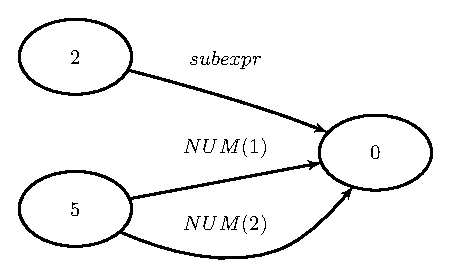
\epsfig{file=graphs/Stack_for_simple_fork.eps}%, height=1.6cm, width=0.8\textwidth}
    \caption{GSS after reduction by the rule $subexpr \rightarrow NUM$.}
    \label{pic5}
\end{figure}


It is important that we suppose that input data structure for parser is DAG with one source and one sink vertices. Our experience of dynamic SQL translation for some real information system shows that DAG is a good approximation of the dynamically constructed expressions set for practical use. We should replace all cycles with single repetition during approximation to get such graph. This way we can process all vertices in the topological order\footnote{Topological sort or topological ordering of a directed graph is a linear ordering of its vertices such that for every directed edge $u \rightarrow v$ from vertex $u$ to vertex $v$, $u$ comes before $v$ in the ordering.}. On each step we should process all outgoing edges for current vertex that leads to Shift/Shift \ ``conflicts'' appearance. As a result we have additional branches in GSS.

We now describe steps of parsing in more details. The grammar, which we use as an example, is shown below.


\begin{verbatim}
s: NUM PLUS e
e: NUM
\end{verbatim}


Input graph is presented in figure~\ref{pic6}.

\begin{figure}
    \centering
    \epsfig{file=graphs/Sum_with_branch.eps, width=0.5\textwidth}
    \caption{Input graph with branching.}
    \label{pic6}
\end{figure}

There are two paths from the start vertex to the final in the input graph: $(0 \rightarrow 1 \rightarrow 3 \rightarrow 4)$ and $(0 \rightarrow 2 \rightarrow 3 \rightarrow 4)$. This paths contain a common subpath $(3 \rightarrow 4)$ which can be reduced to nonterminal \verb X. So we should get SPPF where nodes for nonterminal \verb X \ are common for two trees.


In this part we describe steps of syntax analysis. Vertices of the input graph are processed in the order of topological sort. In one step of the algorithm all outgoing edges of each vertex should be processed. However we only move to stack the edges which are required for the next in order vertex processing. So in case of multiple outgoing edges the algorithm processes only the edge with the tail to be processed the next. The processing of other edges should be postponed. The fact, that each edge will be processed just before processing of the vertex which is the target for this edge, allows to avoid incorrect merging of identical states.  To clarify this we describe stack transformations in greater details.


\begin{table*}
\centering
\caption{States of Parsing Statck}
\begin{tabular}{|c|c|} \hline
        \epsfig{file=graphs/stack/stack1.eps, width=0.5\textwidth}
        \label{A}
&
        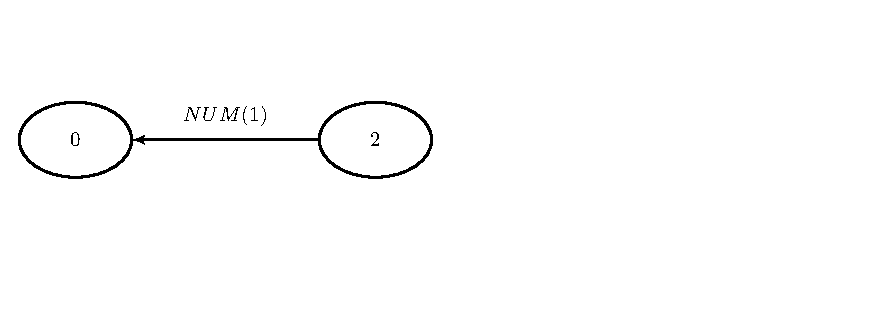
\epsfig{file=graphs/stack/stack2.eps, width=0.5\textwidth}
        \label{B}

\\
A. Start state. & B. First shift.
\\ \hline
        \epsfig{file=graphs/stack/stack3.eps, width=0.4\textwidth}
        \label{C}
&
        \epsfig{file=graphs/stack/stack4.eps, width=0.4\textwidth}
        \label{D}
\\
C. First branch processing is finished. & D. Second brahch processing.
\\ \hline

        \epsfig{file=graphs/stack/stack5.eps, width=0.45\textwidth}
        \label{E}
&
        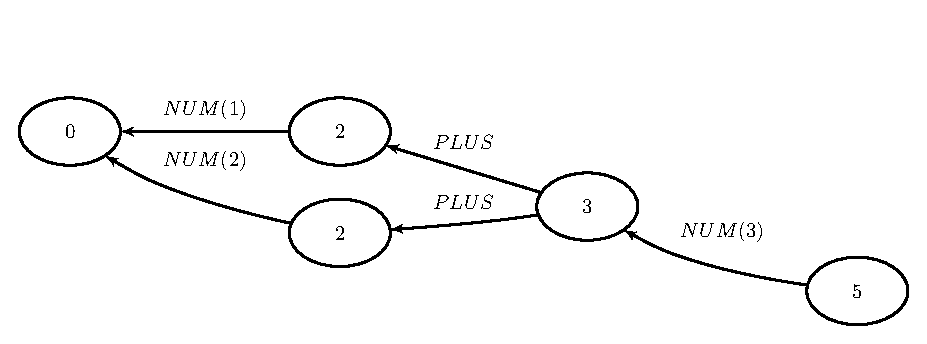
\epsfig{file=graphs/stack/stack6.eps, width=0.45\textwidth}
        \label{F}
\\
E. Second branch processin is finished. & F. Common ``tail'' processing.
\\ \hline

\multicolumn{2}{|c|}{
        \epsfig{file=graphs/stack/stack7.eps, width=0.8\textwidth}
        \label{G}
}

\\

\multicolumn{2}{|c|}{G. Reduction to nonterminal $e$.}

\\ \hline
\multicolumn{2}{|c|}{
        \epsfig{file=graphs/stack/stack8.eps, width=0.8\textwidth}
        \label{H}
}
\\
\multicolumn{2}{|c|}{H. Reduction to nonterminal $s$.} 
\\ \hline

\end{tabular}
\label{tab1}
\end{table*}


During processing of the first vertex with number 0 (figure~\ref{pic6} and table~\ref{tab1}.A) we have branching in the input graph and  Shift/Shift ``conflict''. Vertex with number $1$ is the next vertex in topological order and only token  assigned to the edge $(0 \rightarrow 1)$ is pushed to stack (table~\ref{tab1}.B). So, at first the edges from subpath $(0 \rightarrow 1 \rightarrow 3)$ is processed, and only after that the algorithm processes the edge $(0 \rightarrow 2)$. Because of impossibility of reduction by any rule, the tokens from the path $(0 \rightarrow 1 \rightarrow 3)$ are just pushed into the stack (table~\ref{tab1}.C).


After that all edges from path $(0 \rightarrow 2 \rightarrow 3)$ are processed. In this step a second branch in the stack is arisen. RNGLR-algorithm operates with some property of the vertex called level which determines the order of processing. We redefine the level of the vertex as its number in the topological order. The analyzer merges only the branches tails which have equivalent states and which are on the same level. The last condition guarantees that we avoid false merging of the vertices having equal states but being placed in different paths of an input graph. In our example we should merge the tails of the branches and must not merge the vertices $1$ and $2$ (table~\ref{tab1}.D and table~\ref{tab1}.E). After that, the rest of the graph is processed (table~\ref{tab1}.F -- table~\ref{tab1}.H).


The reductions to the nonterminals $e$ and $s$ are the last steps in the parsing. SPPF construction process is the same as in classical RNGLR.

The resulting SPPF contains two trees corresponding with two paths of the input graph and the subgraph for the nonterminal X is reused (figure~\ref{pic7}).

\begin{figure}
    \centering
    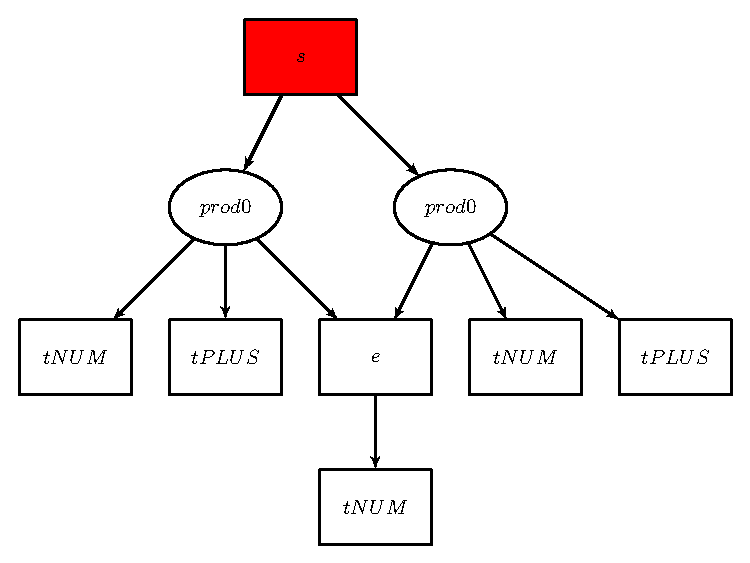
\epsfig{file=graphs/simple_ast.eps, width=0.5\textwidth}

    \caption{Parsing result.}
    \label{pic7}
\end{figure}

\section{Evaluation}

Proposed algorithm of abstract parsing and corresponded parsers generator is implemented as part of YaccConstructor project. Generator allows to create abstract parser by grammar specification. It is implemented as one of modules of YaccConctructor and based on RNGLR parsers generator which  has been implemented previously. A big number of core modules and data structures is reused. So it is possible to generate syntax analyzers for string-embedded languages by the language specification written in one of supported languages such as Yard or FsYacc.

In order to demonstrate the implemented tool let us consider the following grammar:

\begin{verbatim}
binExpr<operand binOp>:operand (binOp operand)*

[<Start>]
expr: binExpr<term termOp>
termOp: PLUS | MINUS
term: res=binExpr<factor factorOp>
factorOp: MULT | DIV
factor: binExpr<powExpr powOp>
powOp: POW
powExpr: n=NUMBER | LBRACE expr RBRACE

\end{verbatim}

The graph shown in figure~\ref{pic8} is used as an input for the syntax analysis.

\begin{figure*}
    \centering
    \epsfig{file=graphs/calc_input_graph.eps, width=0.8\textwidth}
    \caption{Input graph.}
    \label{pic8}
\end{figure*}

The graph shown in figure~\ref{pic9} is a result of the syntax analysis. As you can see, the subtrees corresponded to the common subexpression are re-used. This approach allows to reduce memory consumption in case of large input graphs.

\begin{figure*}
    \centering
    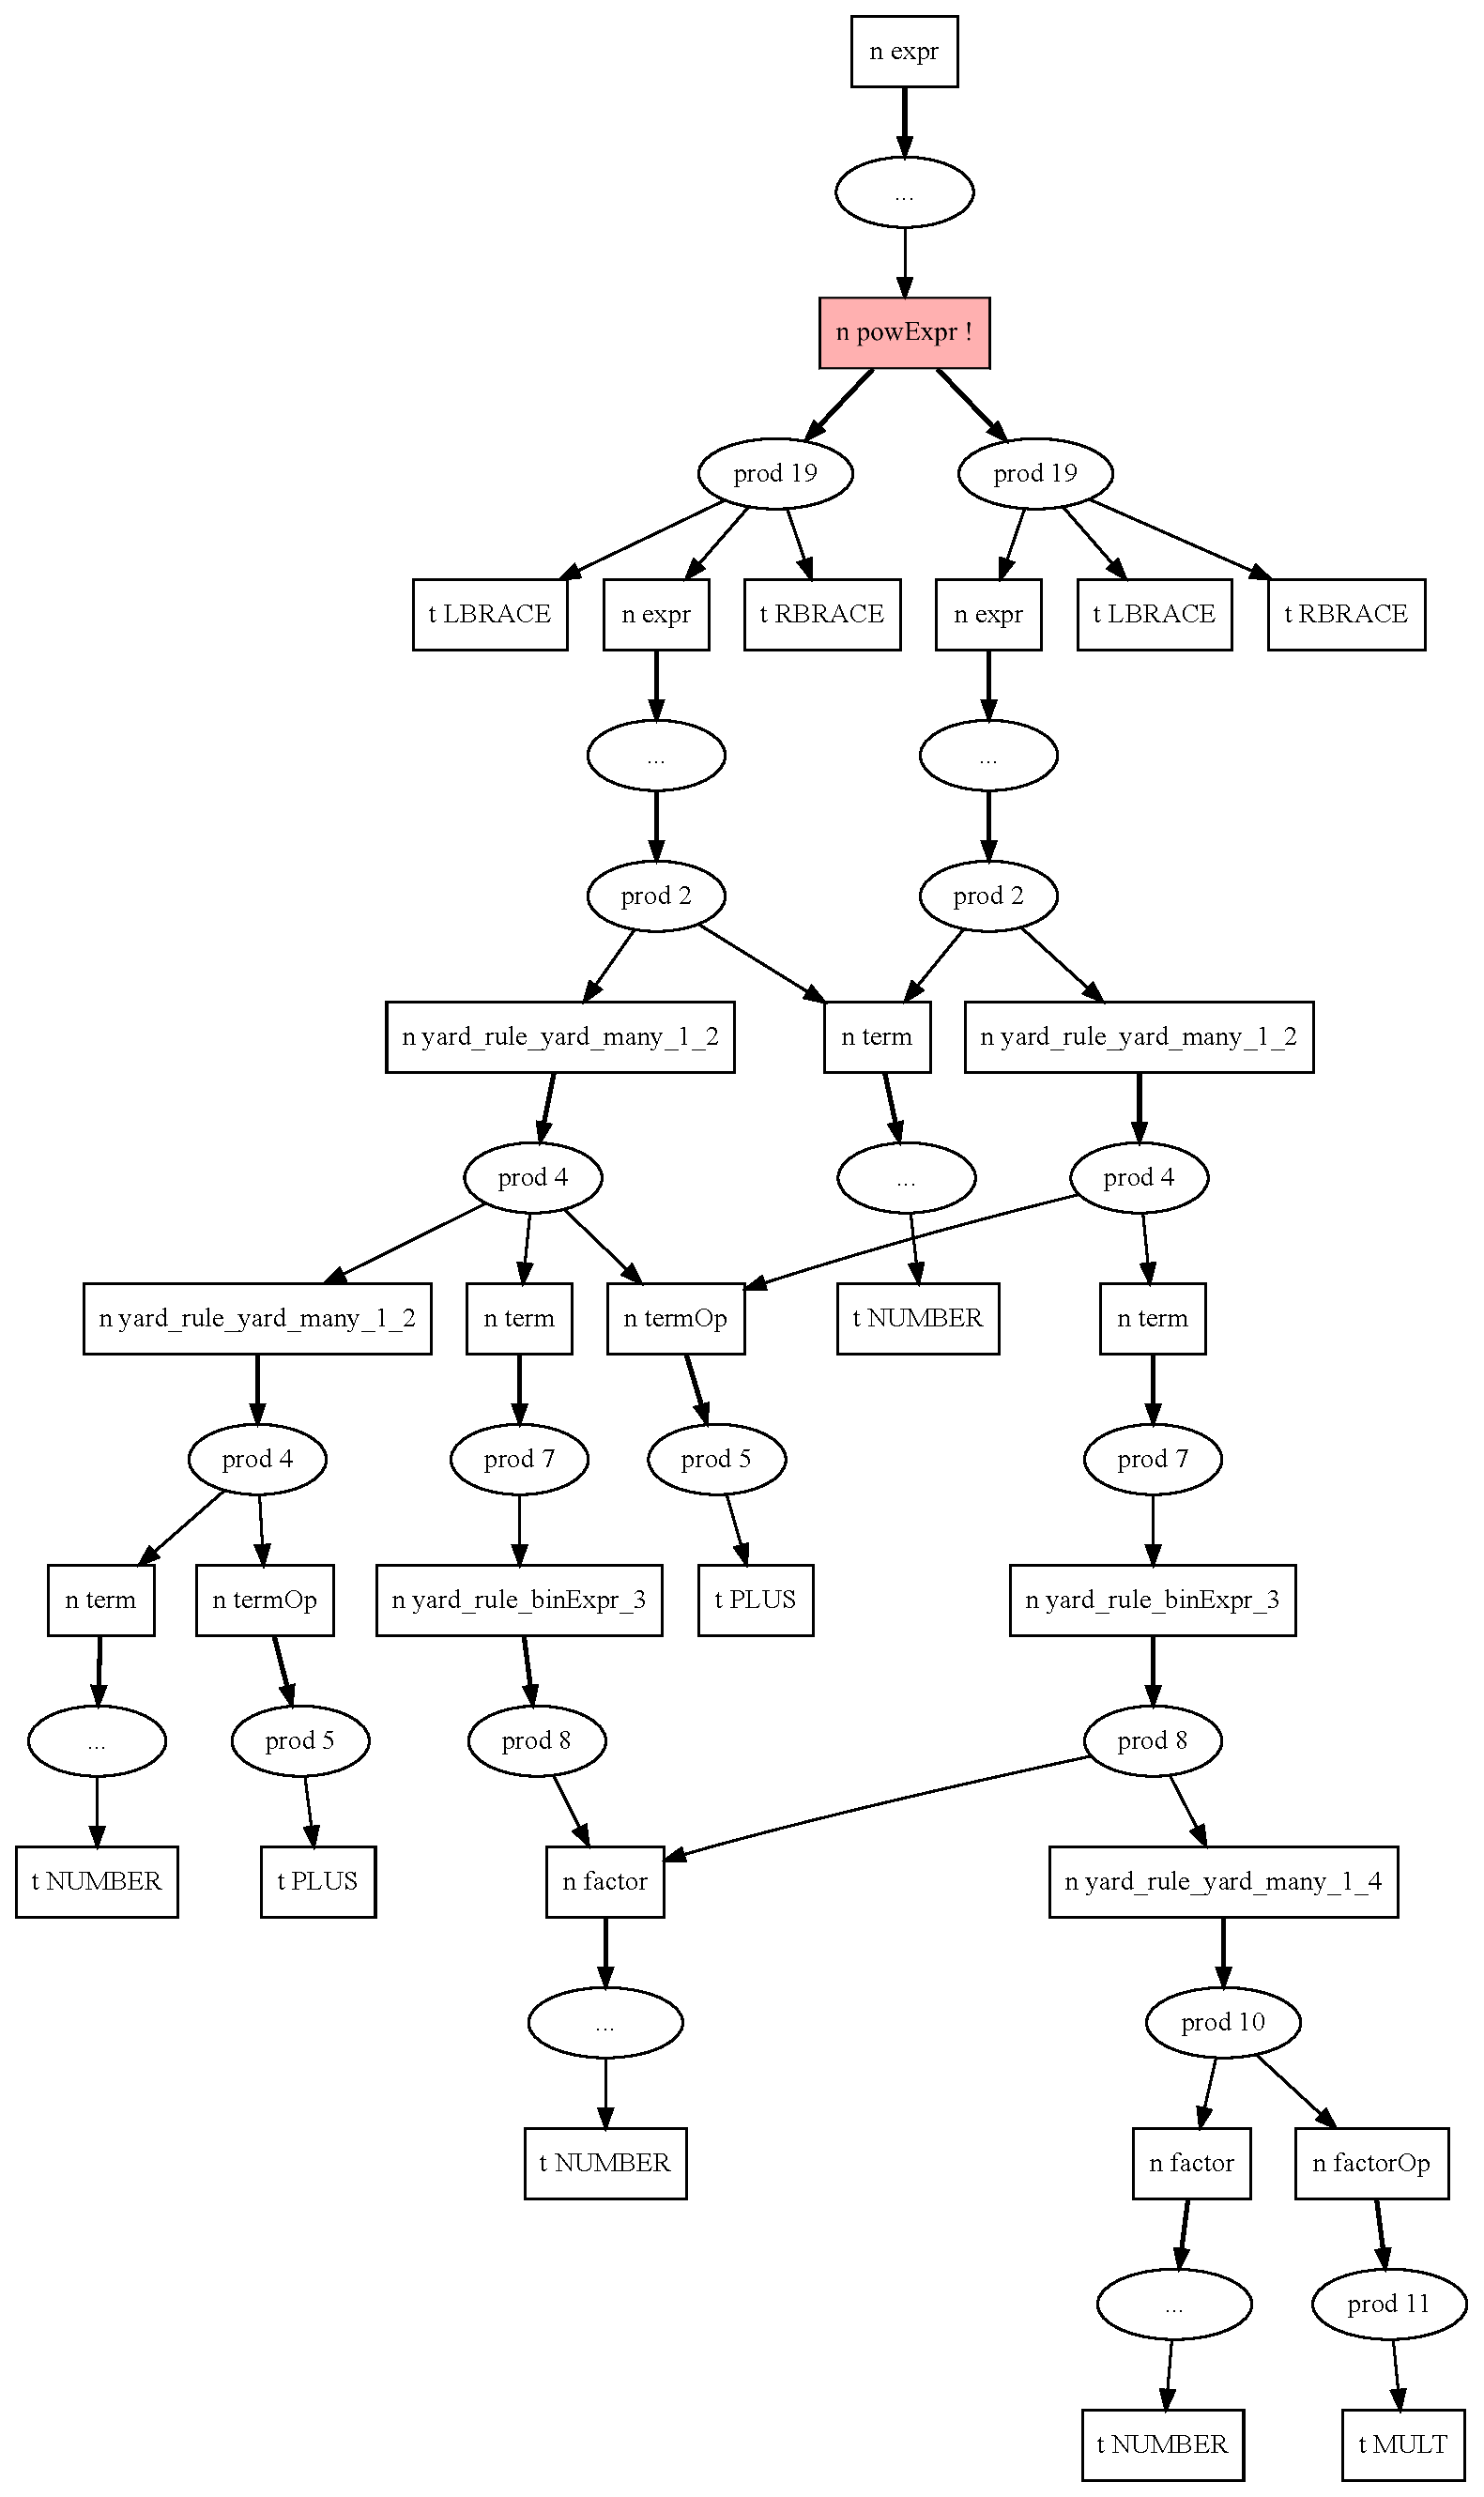
\epsfig{file=graphs/calc_with_branch_3.eps, width=0.8\textwidth}
    \caption{Result of the processing of the graph which presented in figure~\ref{pic8}.}
    \label{pic9}
\end{figure*}



We also have tested the tool as a parser of the T-SQL language subset. The results of the set of performance tests are provided below.

All tests were performed on a PC with following characteristics:
\begin{itemize}
\item OS Name: Microsoft Windows 7 Professional	
\item Version: 6.1.7601 Service Pack 1 Build 7601	
\item System Type: x64-based PC	
\item CPU: Intel(R) Core(TM) i5-2400S CPU @ 2.50GHz, 3201 Mhz, 4 Core(s), 4 Logical Processor(s)	
\item RAM: 16 GB
\end{itemize}

Input data for tests were generated to demonstrate the main cases previously extracted from real-world information system:
\begin{enumerate}
\item Fragments with parallel branches (produced by if-statements or case-statements) sequentially concatenated to a single statement. The most popular example is a select-statement where the name of each field may be calculated within if-statement or case-statement.
\item Nested branches being used for query construction.
\end{enumerate}

An input data for the first case were based on select statement with common prefix and suffix, and fields list which was combined of sequentially concatenated basic blocks with parallel branches. Let $n$ is a number of parallel paths in a basic block and $m$ is a number of blocks. So the number of path in graph is $n^m$. We performed the set of tests for $n \in \{1; 2; 5; 10\}$. For each n the set of graphs with $m \in \{1..52\}$ was generated. The common structure of a graph for $n = N$ and $m = M$ is presented in figure~\ref{pic11}. The example of graph for $n=2$ and $m = 2$ is presented in figure~\ref{pic10}.

\begin{figure*}
    \centering
    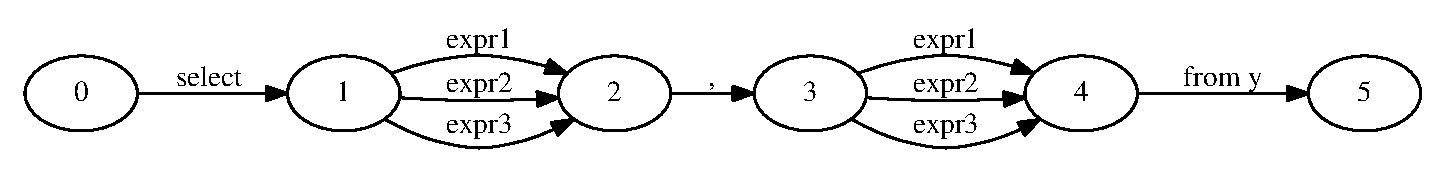
\epsfig{file=graphs/x_10.eps, width=0.8\textwidth}
    \caption{Example of graph with $n=2$ and $m=2$}
    \label{pic10}
\end{figure*}

\begin{figure*}
    \centering
    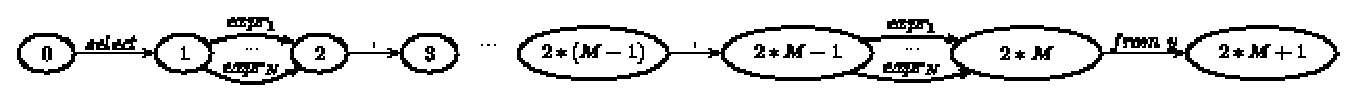
\epsfig{file=graphs/x_10_common_1.eps, width=0.9\textwidth}
    \caption{Common sructure of graph with $n=N$ and $m=M$}
    \label{pic11}
\end{figure*}

So we have a five families of graphs parameterized by $n$. For each family we measure the parsing speed as a function of the number of sequential blocks $m$. Results of tests show that parsing require polynomial time as demonstrated in figure~\ref{pic12} and figure~\ref{pic19}).


\begin{figure}
    \centering
    \epsfig{file=graphics/n5.eps, width=0.5\textwidth}
    \caption{Plotted results of performance tests for case 1, n=5.}
    \label{pic19}
\end{figure}


\begin{figure}
    \centering
    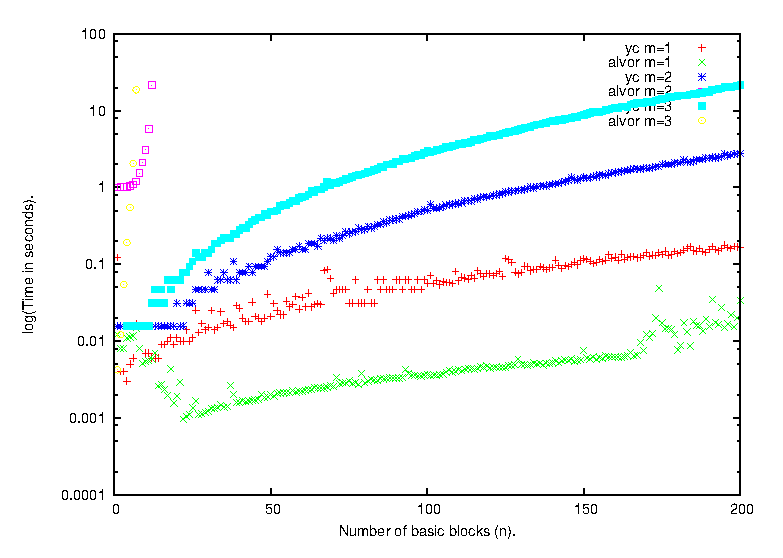
\epsfig{file=graphics/all.eps, width=0.5\textwidth}
    \caption{Plotted results of performance tests for all series in case 1.}
    \label{pic12}
\end{figure}


For the second case (which illustrated conditional branching in a query construction) tests were constructed from recursively nested blocks. All tests had the common prefix \verb SELECT , the common suffix \verb FORM ~ \verb Y, and the list of fields for select which were constructed recursively from basic blocks which contained two vertex and two parallel paths. Let $n$ is a number of test and it specifies the depth of recursion. The list of fields can be generated by the specified number with the function described below.

\begin{verbatim}

let rec nestedBranches n =
    if n = 1
    then basicBlock
    else 
        cond (  expr1 + comma 
              + nestedBranches (n-1) + expr2) 
             (  expr3 + nestedBranches (n-1) 
              + comma + expr4 )
\end{verbatim}

The example of an input graph with $n = 2$ is presented in figure~\ref{pic13}.

\begin{figure*}
    \centering
    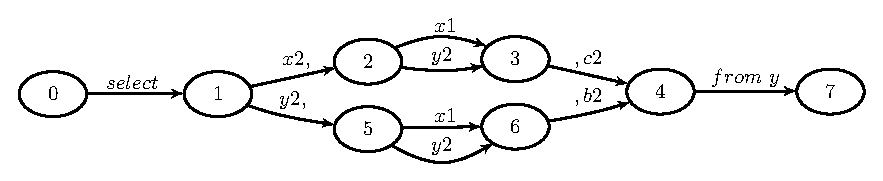
\epsfig{file=graphs/x_8.eps, width=0.8\textwidth}
    \caption{Example of graph for nested branches with $n = 2$.}
    \label{pic13}
\end{figure*}


As a result of the experiments we get that parsing require exponential time. Plotted results of measurements are presented in figure~\ref{pic14}.

\begin{figure}
    \centering
    \epsfig{file=graphics/2n.eps, width=0.5\textwidth}
    \caption{Plotted results of performance tests for case 2.}
    \label{pic14}
\end{figure}



\section{Conclusions and future work}

We created GLR-based algorithm for abstract parsing which reuses graph-structured stack and shared packed parse forest and implemented abstract parsers generator based on this algorithm. We also carried out a series of experiments showing the practical applicability of the generator and the correctness of the implemented modified RNGLR-analyzer.

Plugin for ReSharper\footnote{ReSharper -- developer productivity tool for Microsoft Visual Studio. It's provide powerful code inspections, automated code refactorings, blazing fast navigation, and coding assistance.  \href{http://www.jetbrains.com/resharper/}{http://www.jetbrains.com/resharper/}} based on described algorithm is in active development. This plugin is designed for support of  string-embedded languages in  Microsoft Visual Studio IDE. We are also working on static errors checking in dynamically constructed statements at the current time. The next step is the implementation of the other features of IDE for string-embedded languages such as syntax highlighting, autocompletion and refactorings. Plugin development poses many new questions associated with such problems as incremental regular approximation construction, semantic calculation directly by graph and results caching. Unified modular infrastructure for fast and easy support of new languages is in active development.

In the future, errors handling algorithm should be enhanced and necessity of errors recovery should be investigated.  The fact that input graph may contains a huge number of \ ``incorrect-by-design'' paths makes these questions a bit difficult to answer. It is caused by the fear that errors recovery may produce a big number of inconsistent results.

We also should implement efficient generation of parsing trees from SPPF and user-defined semantic calculation for them. Parallel processing may be used for these tasks but the real usefulness of this approach is a question to be answered by running on the real-world examples. The ambiguity here is caused by the complexity of the data structures for processing. 

One more question is whether it is possible to generalize classical parsing to abstract parsing. Experiments have shown that a generalization is possible but the current implementation causes big performance issues.  Generalized parsing performance is almost 10 times lower than the performance of the classical parsing based on the same algorithm. This may be related to the ineffective implementation of the generalized algorithm or the theoretical limitations. This problem requires an additional investigation.




\bibliographystyle{plain}
\bibliography{bibliography}
\balancecolumns
% That's all folks!
\end{document}
